\documentclass[runningheads]{llncs}
%% The amssymb package provides various useful mathematical symbols
\usepackage{amssymb}
\usepackage{amsmath}
%% The amsthm package provides extended theorem environments
%\usepackage{amsthm}
\usepackage{wrapfig}
\usepackage{lineno}

%% Use package enumitem to align enumeration and itemization
\usepackage{enumitem}
\usepackage{listings}
\usepackage{courier}           % for the courier font (optional)
\usepackage{multicol}          % for two equations side by side
\usepackage[justification=centering]{caption}
\usepackage{xcolor}
\usepackage{stmaryrd}
\usepackage{graphicx}
%\usepackage{url}
\usepackage[misc,geometry]{ifsym} 
\chardef\_=`_

\usepackage[utf8x]{inputenc}
\usepackage[T1]{fontenc}
\usepackage{ae,aecompl}
\PrerenderUnicode{ȘșțȚăĂîÎâÂîÎ}

%\hypersetup{ % play with these to change the look of hyperlinks
%    colorlinks=true,
%    linkcolor=black,
%    filecolor=magenta,
%    urlcolor=cyan,
%   citecolor=black
%}

\colorlet{red}{red!80!black}

%% NEW COMMANDS =============================================

\lstdefinelanguage{Coq}%
  {morekeywords={Notation,Class,Variable,Inductive,CoInductive,Fixpoint,CoFixpoint,%
      Definition,Example,Lemma,Theorem,Axiom,Local,Save,Grammar,Syntax,Intro,%
      Trivial,Qed,Intros,Symmetry,Simpl,Rewrite,Apply,Elim,Assumption,%
      Left,Cut,Case,Auto,Unfold,Exact,Right,Hypothesis,Pattern,Destruct,%
      Constructor,Defined,Fix,Record,Print,Proof,Induction,Hint,Hints,Exists,
      let,in,Parameter,Parameters,Split,Red,Reflexivity,Transitivity,if,then,else,Opaque,%
      Transparent,Inversion,Absurd,Generalize,Mutual,Cases,of,end,Analyze,%
      AutoRewrite,Functional,Scheme,params,Refine,using,Discriminate,Try,%
      Require,Load,Import,Scope,Set,Open,Section,End,match,with,Ltac,%
      exists,forall,fix,fun
	},% 
   keywordstyle=\color{red},%
   basicstyle=\normalfont\small\tt,%
   sensitive, %
   tabsize=2,%
   %escapechar=`,%
   morecomment=[n]{(*}{*)},%
   morestring=[d]",%
   literate={=>}{{$\Rightarrow$}}2 {>->}{{$\rightarrowtail$}}3{<->}{{$\longleftrightarrow$}}3{->}{{$\to$}}2
   {\/\\}{{$\wedge$}}2
   {|-}{{$\vdash$}}2
   {\\\/}{{$\vee$}}2
   {~}{{$\sim$}}1
   %{<>}{{$\neq$}}1 indeed... no.
  }[keywords,comments,strings]%

\lstnewenvironment{coq}{
       \lstset{
        basicstyle=\ttfamily,
        language=Coq,
        showstringspaces=false
       }
}{}
\makeatletter
\newlength{\@mli}
\newcommand{\mli}[1]{%
	\settowidth{\@mli}{\lstinline/#1/}
	\hspace{-.5ex}\begin{minipage}[t]{\@mli}\lstinline/#1/\end{minipage}}
\makeatother
\newcommand{\li}[1]{\ifmmode\mbox{\mli{#1}}\else\mbox{\lstinline/#1/}\fi}

\newcommand\hide[1]{}
\newenvironment{centermath}
{\begin{center}$\displaystyle}
	{$\end{center}}
\renewcommand{\note}[2][polish]{{\color{red} #2}{\marginpar{\tiny \color{blue} #1}}}
\renewcommand{\implies}{\Rightarrow}
\renewcommand{\iff}{\Leftrightarrow}

%\theoremstyle{plain}
%\newtheorem{thm}{Theorem}[section]
%\newtheorem{ex}[thm]{Example}
%\newtheorem{prop}[thm]{Proposition}
%\newtheorem{col}[thm]{Corollary}
%\newtheorem{lem}[thm]{Lemma}
%\newtheorem*{hypo}{Hypothesis}
%\theoremstyle{definition}
%\newtheorem{defn}[thm]{Definition}
%\newtheorem{rem}[thm]{Remark}

%\crefname{thm}{theorem}{theorems}
%\crefname{defn}{definition}{definitions}
%\crefname{lem}{lemma}{lemmas}
%\crefname{col}{corollary}{corollaries}
%\crefname{ex}{example}{examples}
%\crefname{prop}{proposition}{propositions}

%\Crefname{thm}{Theorem}{Theorems}
%\Crefname{defn}{Definition}{Definitions}
%\Crefname{lem}{Lemma}{Lemmas}
%\Crefname{col}{Corollary}{Corollaries}
%\Crefname{ex}{Example}{Examples}
%\Crefname{prop}{Proposition}{Propositions}

%% DOCUMENT =================================================

\bibliographystyle{plainurl}% the mandatory bibstyle

\begin{document}
	
\title{Formalizing Correct-By-Construction Casper \\ in Coq}

\author{Elaine Li\inst{1}, Traian \textcommabelow{S}erbănu\textcommabelow{t}ă\inst{1}, Denisa Diaconescu\inst{1}, Grigore Ro\textcommabelow{s}u\inst{1}, Vlad Zamfir\inst{2}}
\institute{Runtime Verification \\ 
					\and 
					Ethereum Research\\}

\maketitle

\begin{abstract}
We present a machine-checked formalization of the Correct-By-Construction Casper family of consensus protocols (CBC Casper) using the Coq proof assistant. 
We leverage Coq's type classes to represent CBC Casper at various levels of abstraction. 
We construct a type class hierarchy showing the relationship between the various abstractions and the properties they derive. 
In doing so, we 1) illuminate the assumptions that each property depend on, and 2) reformulate the protocol in general, mathematical terms. 
We highlight two advantages of our approach: 1) from a proof engineering perspective, it enables a clean separation of concerns between theory and implementation; 2) from a protocol engineering perspective, it provides a rigorous, foundational understanding of the protocol which is conducive towards finding and proving stronger properties. We detail one such new property, namely strong non-triviality. 
\end{abstract}

\section{Overview} 
In the first section we give an account of the motivating principles behind our formalization of CBC Casper, and the design choices they give rise to. For a motivation of CBC Casper at large, we refer the reader to \cite{CBCfull}. 

In the second section we describe our formalization. We present our abstraction hierarchy, with each level consisting of a type class containing a collection of parameters and axioms. We explicate 1) how the levels relate to one another, and 2) how desirable protocol properties such as safety, consistency and non-triviality are derived from each level. 

In the third section we present formalizations of two concrete protocols: a full node and light node version of CBC Casper, as described in \cite{CBCfull} and \cite{CBClight} respectively. We show how our concrete definitions instantiate an abstract type class. We highlight parameters in the type class that are instantiated differently between the full and light node versions, and explain how this reflects the essential differences between the protocols. In doing so, we illustrate how using type classes as an abstraction mechanism allows us to separate concerns between theory and implementation. 

In the fourth section we present a new proof of a protocol property which we call strong non-triviality, for both the full node and light node protocols. We highlight how our abstraction hierarchy invites a precise mathematical characterization of CBC Casper, which paves the way for us to look for and prove stronger properties. We discuss our ongoing attempts at refining our abstraction hierarchy. 

In the final section, we discuss related work, and conclude. 


\section{Design choices} 
A salient feature of the CBC Casper family of protocols, as captured in its ``correct-by-construction'' namesake, is that desirable protocol properties such as safety and consistency should be guaranteed independently of its choice of parameters. However, these properties do rely on certain implicit or explicit assumptions about the parameters that can be used to fully specify any protocol. Our primary aim was to thoroughly investigate CBC Casper's protocol properties and the assumptions they depend on, by abstracting away from protocol-specific language and characterizing the properties and their assumptions in general mathematical terms. We took an incremental approach: starting with the existing description of partially-specified protocols and their properties, we progressively parameterized protocol features such as state definitions, the notion of equivocation, and reachability, and observed which properties would no longer hold. This process allowed us to precisely pinpoint the minimal assumptions required for each desirable property. 

We found Coq's type classes to be a suitable abstraction to present our findings. Our reasons are twofold: 1) the relationship between type class and instances of it aptly reflects the relationship between CBC Casper and its members; 2) Coq's type inference mechanism allows us to organize typeclasses in relation to one another and thereby elucidate the relationship between assumptions and properties. We present the our formal abstraction using type classes in the following section. 

\section{Formalization}
\label{sec:formalization}

\subsection{Parameters}
Each member of the CBC Casper protocol family is identified by five parameters, namely validators, validator weights, consensus values, the estimator function, and a fault tolerance threshold \cite{CBCfull}. Each of these parameter satisfies certain explicit properties, such as non-negativity for validator weights and the fault tolerance threshold, totality for the estimator function etc. We model these parameters as-is, as generic \verb|Type|s in Coq, accompanied by explicit statements of their additional properties. 

\subsubsection{Validators} 
Validators represent the consensus-forming nodes in the protocol. We require of validators the fact that 1) they form a non-empty set, namely that there is at least one validator, and 2) they are comparable. We capture both of these requirements in a generic type class \verb|StrictlyComparable|, which is parameterized by an abstract type \verb|X|. 
\begin{coq}
	Class StrictlyComparable (X : Type) : Type :=
	{
		inhabited : exists (x : X), True;
		compare : X -> X -> comparison;
		compare_strictorder :> CompareStrictOrder compare;
	}.
\end{coq}
\verb|StrictlyComparable| contains a proof that there exists at least one witness of type \verb|X| (\verb|inhabited|), a comparison operator which takes two elements of type \verb|X| and returns either \verb|Lt|, \verb|Eq| or \verb|Gt| (\verb|compare|), and a proof that this comparison operator imposes a strict ordering on elements of type \verb|X|, i.e. that it is both reflexive and transitive (\verb|compare_strictorder|). 
This is reflected in the type class as follows: 
\begin{coq}
	validators : Type; 
	about_validators : StrictlyComparable validators;
\end{coq}
\subsubsection{Validator weights} 
Validator weights are computed by a function which takes a validator name and returns a positive real number. We represent positive real numbers using dependent types in Coq, and represent the validator weight function with the following function signature: 
\begin{coq}
	weight : validators -> {r | (r > 0)%R};
	\end{coq}
\subsubsection{Consensus values} 
The requirements for consensus values represented as abstract types are similar to those for validators. 
\begin{coq}
	consensus_values : Type; 
	about_consensus_values : StrictlyComparable consensus_values; 
\end{coq}
\subsubsection{Estimator} 
The estimator function is a total function which takes a state and returns a non-empty set of consensus values. We represent the estimator function using a relation of type \verb|state -> consensus_values -> Prop|, which can be interpreted as an assertion that the estimator agrees on some consensus value for some state. We assume for now, as in \cite{CBCfull}, that we have some notion of states. 
\begin{coq}
	E : state -> consensus_values -> Prop; 
	estimator_total : forall s, exists c, E s c; 
\end{coq}
\subsubsection{Fault tolerance threshold} 
The Byzantine-fault tolerance threshold is a non-negative real number that is strictly smaller than the sum of all validator weights. Because Coq \verb|Type|s are not guaranteed finite, we state the strictly smaller requirement in terms of the existence of a finite list of validators whose sum exceeds the fault weight. 
\begin{coq}
	t : {r | (r >= 0)%R}; 
		suff_val : exists vs,  NoDup vs /\ 
		((fold_right (fun v r=>(proj1_sig (weight v) + r)%R) 0%R) vs 
		> (proj1_sig t))%R;
\end{coq}

The full node specification of CBC Casper, given in \cite{CBCfull}, features a mutually recursive definition of states and messages. States are defined as ``\textit{certain} sets of messages'', while messages are defined as ``\textit{certain} triples of the form (consensus value, validator name, protocol state)''. Correspondingly, a light node specification of a CBC Casper, given in \cite{CBClight}, features a slightly different definition of states and messages that is not as strongly mutually recursive. Both specifications satisfy three cornerstone safety theorems. Therefore, our first level of abstraction parameterizes the definition of states, and abstracts away messages. 

\subsubsection{States} 
We define a preliminary abstract state type, \verb|state|. We similarly require that these states are \verb|StrictlyComparable|. We define an initial state, \verb|state0| of type \verb|state|. We additionally define an abstract notion of state equality and a commutative state union operator. 
\begin{coq}
	state : Type;
	about_state : StrictlyComparable state;
	state0 : state;
	state_eq : state -> state -> Prop;
	state_union : state -> state -> state;
	state_union_comm : forall s1 s2, state_eq (state_union s1 s2) 
	(state_union s2 s1);
\end{coq}
Further, we define a reachability relation on abstract states. We require of this reachability relation that it is reflexive and transitive. We relate reachability with the state union operator with the requirement that any state is able to reach its union with any other state. Finally, we require that reachability respects state equality. 
\begin{coq}
	reach : state -> state -> Prop;
	reach_refl : forall s, reach s s; 
	reach_trans : forall s1 s2 s3, reach s1 s2 -> 
	reach s2 s3 -> 
	reach s1 s3; 
	reach_union : forall s1 s2, reach s1 (state_union s1 s2);  
	reach_morphism : forall s1 s2 s3, reach s1 s2 -> 
	state_eq s2 s3 -> 
	reach s1 s3;  
\end{coq}

\subsubsection{Protocol states}
We represent restricting elements of generic type \verb|state| to valid protocol states by defining protocol state as a property of type \verb|state -> Prop|. In this way, we fully abstract the mutually recursive definition of states, messages and protocol states into the implementation layer. We require of the property \verb|prot_state| that it holds for the initial state. 
\begin{coq}
	prot_state : state -> Prop; 
	about_state0 : prot_state state0; 
\end{coq}

\subsubsection{Equivocation} 
Finally, we abstract away the details of computing fault weight from states by representing the fault weight of a state as a function of type \verb|state -> R|. We require that the fault weight of the union of two states is greater than or equal to the fault weight of each individual state, and we relate the definition of protocol states with fault weight by requiring that two protocol states' union is a protocol state iff its fault weight is under threshold. 
\begin{coq}
	equivocation_weight : state -> R; 
	equivocation_weight_compat : forall s1 s2, 
	(equivocation_weight s1 <= 
	equivocation_weight (state_union s2 s1))%R; 
	about_prot_state : forall s1 s2, 
	prot_state s1 -> prot_state s2 ->
	(equivocation_weight (state_union s1 s2) 
	<= proj1_sig t)%R  -> 
	prot_state (state_union s1 s2);
\end{coq}
This completes the parameters and axioms included in our first abstraction layer, which we call \verb|CBC_protocol_eq|. Next, we show how this abstraction layer derives all the asynchronous, Byzantine-fault tolerant consensus safety theorems for CBC Casper. 

\subsection{Safety} 
CBC Casper protocols satisfy three key safety properties, namely 1) common futures, 2) consistency of decisions on protocol states, and 3) consistency of decisions on consensus values. In each of the following proofs, we assume that we have a generic instance of the type class \verb|CBC_Casper_eq|. 
\subsubsection{Common futures} 
We prove that protocol states have common futures as long as their union state is a valid protocol state. We proceed stepwise, as in \cite{CBCfull}: first we show that any pair of protocol states satisfies the common futures property, then we use it to generalize to an arbitrary number of states. 
\begin{coq}
	Theorem pair_common_futures '{CBC_protocol_eq}:
	forall s1 s2 : pstate,
	(equivocation_weight (state_union s1 s2) <= proj1_sig t)%R ->
	exists s : pstate, pstate_rel s1 s /\ pstate_rel s2 s.
	
	Theorem n_common_futures "{CBC_protocol_eq} :
	forall ls : list pstate,
	(equivocation_weight (fold_right state_union state0 (map (fun ps => proj1_sig ps) ls)) 
	<= proj1_sig t)%R ->
	exists ps : pstate, Forall (fun ps' => pstate_rel ps' ps) ls.
\end{coq}	

\subsubsection{Consistency of decisions on protocol states}
We prove that protocol states which have common futures cannot make conflicting decisions on future states. We again proceed stepwise, first showing that any two protocol states with a common future cannot make conflicting decisions on future states. 
\begin{coq}
	Theorem pair_consistency_prot '{CBC_protocol_eq} :
	forall s1 s2 : pstate,
	(equivocation_weight (state_union s1 s2) <= proj1_sig t)%R ->
	forall P, 
	~ (decided P s1 /\ decided (not P) s2).
\end{coq}
We then generalize this result to an arbitrary number of states. We first generalize the definition of consistent decisions to a list of states. 
\begin{coq}
	Definition state_consistency '{CBC_protocol_eq} 
	(ls : list pstate) : Prop :=
	exists s : pstate,
	forall (P : pstate -> Prop),
	Exists (fun s => decided P s) ls ->
	P s.
\end{coq}
We then state n-party consensus value consistency as follows: 
\begin{coq}
	Theorem n_consistency_prot '{CBC_protocol_eq} :
	forall ls : list pstate,
	(equivocation_weight (fold_right state_union state0 
	(map (fun ps => proj1_sig ps) ls)) <= proj1_sig t)%R ->
	state_consistency ls.
\end{coq}

\subsubsection{Consistency of decisions on consensus values} 
Showing that protocol states which have common futures cannot make conflicting decisions on consensus values follows naturally from the fact that consensus values are parameterized by state. The statement of consensus value safety is as follows: 
\begin{coq}
	Theorem n_consistency_consensus '{CBC_protocol_eq} :
	forall ls : list pstate,
	(equivocation_weight (fold_right state_union state0 
	(map (fun ps => proj1_sig ps) ls)) <= proj1_sig t)%R ->
	consensus_value_consistency ls. 
\end{coq}

\subsection{Partial order}
With \verb|CBC_protocol_eq| as a starting point, we found that it was possible to further abstract away protocol-specific parameters while preserving the desired safety properties, albeit in more abstract terms. One particular abstraction we explored was a partial order, formally defined as follows: 
\begin{coq} 
	Class PartialOrder :=
	{ A : Type;
		A_eq_dec : forall (a1 a2 : A), {a1 = a2} + {a1 <> a2};
		A_inhabited : exists (a0 : A), True; 
		A_rel : A -> A -> Prop;
		A_rel_refl :> Reflexive A_rel;
		A_rel_trans :> Transitive A_rel;
	}.
\end{coq} 	
We found that valid protocol states in CBC Casper protocols along with future reachability could be represented as a partial order, with the join of two states corresponding to protocol state union, and existing iff it did not exceed the fault tolerance threshold. We formally show this by proving that CBC Casper type class \verb|CBC_protocol_eq| can instantiate a \verb|PartialOrder| type class: 
\begin{coq}
	Instance level0 `{CBC_protocol_eq} : PartialOrder :=
	{ A := pstate;
		A_eq_dec := pstate_eq_dec;
		A_inhabited := pstate_inhabited;
		A_rel := pstate_rel;
		A_rel_refl := pstate_rel_refl;
		A_rel_trans := pstate_rel_trans;
	}.
\end{coq}
We summarize our abstraction hierarchy for CBC Casper in the diagram below. Boxes represent type classes, and ovals represent properties. Solid arrows between type classes represent ``instantiate'', and dotted arrows between type classes and properties represent ``derive''. All arrows are transitive, meaning that \verb|FullNode| and \verb|LightNode| also derive safety properties because they instantiate \verb|PartialOrder|. We note that although we state safety properties in terms of the \verb|CBC_protocol_eq| type class above, the safety properties can be stated in more general terms using just a partial order. Definitions of the boxes and proofs of the solid arrows in this diagram can be found in \verb|protocol.v|. 
\begin{figure}
	\centering
	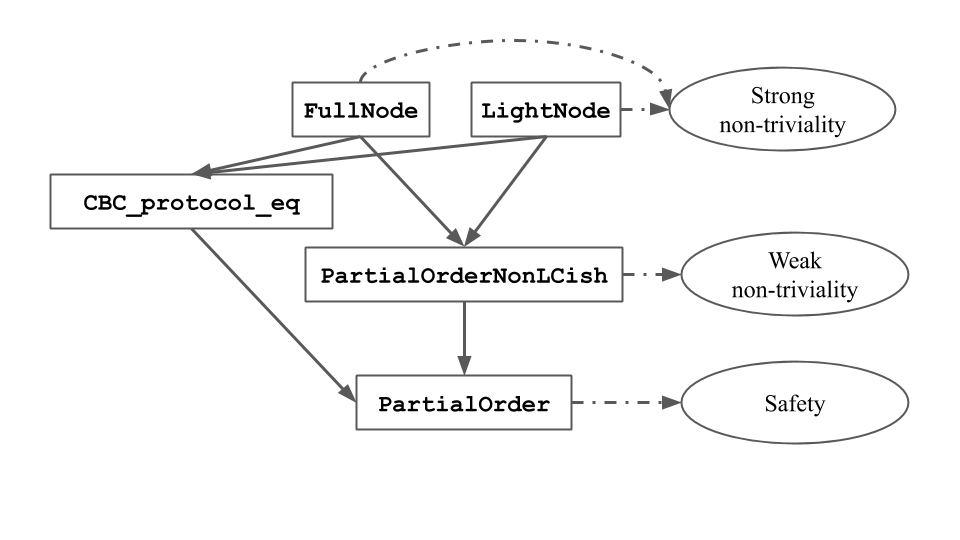
\includegraphics[scale = 0.3]{Flowchart.png}
	\caption{Type class hierarchy representing relationship between type classes and derived properties}
	\label{fig:flowchart}
\end{figure}

In the following sections, we present the key ingredients of our formalization of \verb|FullNode| and \verb|LightNode|. The full instantiation from \verb|FullNode| and \verb|LightNode| to \verb|CBC_protocol_eq| can be found in \verb|fullnode.v| and \verb|lightnode.v| respectively. 

\section{Full node} 
\label{sec:full}
\subsection{States, messages, representatives}

The full-node protocol states are {\em sets} of messages,
each message being a triple $(c, v, j)$, where:
\begin{itemize}
    \item $c$ is a (proposed) consensus value
    \item $v$ identifies the sender of the message
    \item $j$, the justification, {\em is the protocol state} in which the sender
        was at the time the message was sent
\end{itemize}

There are two technical difficulties with the above definition:  
\begin{itemize}
    \item It is recursive (states are sets of messages, each containing a state)
    \item The ordering of the message should not matter
\end{itemize}

To solve the first issue, we chose to postpone the definition of messages and
to define states inductively as follows:

\begin{coq}
Inductive state : Type :=
  | Empty : state
  | Next : C ->  V -> state -> state -> state.
\end{coq}

This definition says that a state can be build by extending an existing state
given a consensus value (C), a validator (V), and another state representing
the justification.
To clarify that the three are the components of a message, we introduce the
following notation for \verb"Next":

\begin{coq}
Notation "'add' ( c , v , j ) 'to' sigma" :=
  (Next c v j sigma)
  (at level 20).
\end{coq}

This definitions addresses the first issue mentioned above, that is, the 
recursive nature of states.

The second issue is very important as it relates to the notion of
state equality.
Although it is pottentially possible to define an equivalence between
states which disregards the order between messages, that is definitely
not trivial, because it is itself recursive, as it requires an equivalence
on messages, which must be defined in terms of the same state equivalence.
This would be a hinderance to both define it and work with it.

Our approach was to work with canonical representatives of these classes,
namely what we called LocallySorted states.  Although this definition
is still recursive, it's easier to express and to work with it than with the
equivalence one because it is only defined in terms of a single state.

To define the notion of sorted states, we need to be able to compare messages,
which amounts to defining a (total) order relation on states.
This can be defined as a lexicographic ordering on the state seen as a list
of messages, with the tweak of recursing in order to compare justifications:

\begin{coq}
Fixpoint state_compare (sigma1 sigma2 : state) : comparison :=
  match sigma1, sigma2 with
  | Empty, Empty => Eq
  | Empty, _ => Lt
  | _, Empty => Gt
  | add (c1, v1, j1) to sigma1, add (c2, v2, j2) to sigma2 =>
    match compare c1 c2 with
    | Eq =>
      match compare v1 v2 with
      | Eq =>
        match state_compare j1 j2 with
        | Eq => state_compare sigma1 sigma2
        | cmp_j => cmp_j
        end
      | cmp_v => cmp_v
      end
    | cmp_c => cmp_c
    end
  end.
\end{coq}

Note that defining this ordering requires a existing orderings on
consensus values and validators, but these can any orderings,
and an total ordering is guaranteed to exists for any set in set theory
including axiom of choice\footnote{Dense orderings, partitions and weak
forms of choice, by Carlos G. Gonzalez FUNDAMENTA MATHEMATICAE 147 (1995)}.
    
This ordering naturally induces an ordering on messages, and thus allows us
to define the notion of a \verb"LocallySorted" state, i.e., one in which
each message is smaller than the next and all justifications are themselves
\verb"LocallySorted".

\verb"LocallySorted" states are chosen as representatives for states, with the
benefit that testing equality of such states reduces to checking syntactic
equality.

Protocol states are defined by means of an inductive predicate on states, by

\begin{coq}
(* Valid protocol state definition *) 
Inductive protocol_state : state -> Prop :=
  | protocol_state_empty : protocol_state Empty
  | protocol_state_next
         : forall s j
         , protocol_state s
        -> protocol_state j
        -> incl_messages j s
        -> forall c v
         , valid_estimate c j
        -> not_heavy (add_in_sorted_fn (c,v,j) s)
        -> protocol_state (add_in_sorted_fn (c,v,j) s).
\end{coq}

The above definition reads as:
\begin{itemize}
    \item a protocol state is either empty; or
    \item it can be obtained from an existing protocol state $s$ by extending
        it with a message $(c, v, j)$ such that:
        \begin{itemize}
            \item $j$ is a protocol state included in $s$
            \item $c$ is a consensus values which can be estimated by $j$
            \item adding $(c,v,j)$ to $s$ does not produce a heavy state
        \end{itemize}
\end{itemize}

\subsection{Strong-non-triviality proofs}
Emphasis on explicating: 
\begin{enumerate}
	\item strong non-triviality proof: atomic equivocation construction, pivotal validator proof, recursive atomic equivocation construction, overall proof sketch
\end{enumerate}




\section{Light node}
\label{sec:light}
\subsection{States, hashes, messages, representatives}

The light-node protocol states are also sets of messages,
each message being a triple $(c, v, j)$, where:
\begin{itemize}
    \item $c$ is a (proposed) consensus value
    \item $v$ identifies the sender of the message
    \item $j$, the justification, is the {\em set of hashes} of all messages
        of the protocol state in which the sender was at the time the message
        was sent
\end{itemize}

The fact that justification is a set of hashes allows for a simpler,
non-recursive definition. To begin, the type of hashes can be any
totally ordered set, a justification can be a list of hashes, and
a message is now just a triple:

\begin{coq}
Variable hash : Type.
Variable (about_H : `{StrictlyComparable hash}). 

Definition justification_type : Type := list hash. 

Definition message : Type := C * V * justification_type.
\end{coq}

The total order on hashes induces a total lexicographic order on
justifications, which can be extended to messages.

We therefore can work with sorted lists of hashes as representatives
for sets of hashes, reducing equality between justifications to
syntactic equality.

For states we prefer to define equality as set-equality, that is
double inclusion between the sets of messages representing states.

Assuming an injective function from messages to hashes,
\begin{coq}
Parameters (hash_message : message -> hash)
           (hash_message_injective : Injective hash_message).
\end{coq}    
we can recursively define a function \verb"hash_state" taking 
states to sorted lists of hashes, i.e., justifications, with the
property that two justifications are equal iff they belong to 
states which are equal as sets:

\begin{coq}
Lemma hash_state_injective : forall sigma1 sigma2,
  hash_state sigma1 = hash_state sigma2
  <->
  set_eq sigma1 sigma2.
\end{coq}    

This allows for the following inductive definition of protocol states:

\begin{coq}
Inductive protocol_state : state -> Prop :=
| protocol_state_nil : protocol_state state0
| protocol_state_cons : forall (j : state),
    protocol_state j ->
    forall (c : C),
      valid_estimate c j ->
      forall (v : V) (s : state),
        In (c, v, hash_state j) s ->
        protocol_state (set_remove compare_eq_dec (c, v, hash_state j) s) ->
        NoDup s ->
        not_heavy s ->
        protocol_state s.
\end{coq}

The above definition reads as:
\begin{itemize}
    \item a protocol state is either empty; or
    \item it is a non-heavy, non-duplicate state $s$ for which
        there exist a consensus value $c$, a sender $V$, and a state $j$ such that:
        \begin{itemize}
            \item $j$ is a protocol state
            \item $c$ is a consensus values which can be estimated by $j$
            \item $(c,v, \texttt{hash\_state}\  j)$ belongs to $s$
            \item The state obtained from $s$ by removing
                $(c,v, \texttt{hash\_state}\  j)$ is a protocol state.
        \end{itemize}
\end{itemize}



\section{Strong non-triviality} 
In this section we pivot to another class of consensus protocol properties, namely non-triviality. \cite{CBClight} uses the notion of non-triviality of protocol properties to illustrate the significance of restricting valid protocol states to those that are not too heavy, i.e. those whose equivocation weights do not exceed the fault tolerance threshold. \cite{CBClight} defines non-triviality as the existence of a protocol property $P$ for which there is a protocol state $sigma_1$ that is decided on $P$ and another protocol state $sigma_2$ that is decided on $\neg P$. 
In our generalization efforts, we found that non-triviality precisely captures the notion of non-local confluence in the abstract rewriting system literature, and can be expressed as follows: 
\begin{coq}
Class PartialOrderNonLCish `{PartialOrder} :=
	{ no_local_confluence_ish : exists (a a1 a2 : A),
		A_rel a a1 /\ A_rel a a2 /\
		~ exists (a' : A), A_rel a1 a' /\ A_rel a2 a';
	}.
\end{coq}
Naturally, the question of whether we could strengthen the first existential quantifier to a universal quantifier arose. We found a positive answer to this question, and further found that the \verb|A_rel a a1| could be strengthened from generic reachability to atomic reachability, i.e. the statement holds when \verb|a| reaches \verb|a1| in one step. We state this strengthened version of non-triviality, which we call strong-nontriviality, as follows: 
\begin{coq}
Definition strong_nontriviality :=
	forall (s1 : pstate),
	exists (s2 : pstate),
	next_future s1 s2 /\
	exists (s3 : pstate),
	yes_common_future s1 s3
	/\
	no_common_future s2 s3. 
\end{coq}
Strong non-triviality states that for every protocol state \verb|s1|, there exists a protocol state \verb|s2| that is \verb|s1|'s next state and a protocol state \verb|s3| that is \verb|s1|'s future state, such that \verb|s1| and \verb|s3| share a common future, but \verb|s2| and \verb|s3| do not. 
In the following section, we explicate our proof of strong non-triviality. While we can instantiate \verb|PartialOrderNonLCish| with our full node and light node protocol definitions, we cannot prove that our abstract CBC Casper type class \verb|CBC_protocol_eq| can directly instantiate a \verb|PartialOrderNonLCish| type class because additional assumptions are required. 
Nevertheless, we observe that the proof of strong non-triviality follows a general abstract pattern shared between the full and light node versions. Pinpointing the precise additional assumptions is topic of ongoing work. Thus, we follow the same approach we used to explicate \verb|CBC_protocol_eq| above: we first give an abstract proof sketch which highlights similarities to the fullest extent; we then go into the details of the specific proof for full and light node, highlighting the differences between them. 

\subsection{Proof sketch} 
By definition, valid protocol states are states that do not exceed the fault tolerance threshold, in other words, states that do not admit too many equivocating senders (recall the definition of \verb|fault_weight_state| in Section \label{sec:formalization} above). Since validator weights are discrete, senders can continue to equivocate, increasing the state's fault weight, until we reach a state that is on the verge of exceeding the fault weight, i.e. states that cannot admit anymore equivocating senders. These states are non-locally confluent: if an additional equivocating sender sends a pair of equivocating messages from that state, the resulting two states can never join. We call these states heavy states, and we call the additional equivocating sender a pivotal sender. We formalize this notion of a pivotal sender with regards to some heavy state as follows. We note that a heavy state can have multiple pivotal senders, but for the purposes of proving strong non-triviality it suffices to show the existence of one.
\begin{coq}
Definition potentially_pivotal_state (v : definitions.V) 
																		 (s : state) :=
	~ In v (equivocating_senders s) /\
	exists (vs : list definitions.V),
	NoDup vs /\
	~ In v vs /\ 
	(forall (v : definitions.V), 
	In v vs -> ~ In v (equivocating_senders s)) /\
	(sum_weights ((equivocating_senders s) ++ vs) 
	<= proj1_sig t_full)%R /\
	(sum_weights ((equivocating_senders s) ++ vs) >
	proj1_sig t_full - proj1_sig (weight v))%R. 
\end{coq}
Formally, we say that \verb|v| is a pivotal sender for some state \verb|s| iff 1) \verb|v| is not already seen to be equivocating in \verb|s|, and there exists a remaining set of validators \verb|vs| which 2a) does not contain \verb|v| and 2b) that are all not already seen to be equivocating in \verb|s|, that 2c) tip over the fault weight of \verb|s| only with the help of \verb|v|. We include an explicit duplicate-free requirement for \verb|vs| because we represent sets using inductively-defined lists in Coq, which do not automatically come with this property. 
We then prove that every protocol state has such a pivotal sender: 
\begin{coq}
Lemma all_pivotal_validator :
	forall (s : state),
	protocol_state s -> 
	exists (v : definitions.V),
	potentially_pivotal_state v s. 
\end{coq}
Based on this critical property of protocol states, we can prove strong non-triviality as per our formal statement above as follows: given an arbitrary protocol state \verb|s1|, we can obtain from \verb|all_pivotal_validator| a set of validators \verb|vs| and a single pivotal validator \verb|v| with special properties above. We can construct a pair of equivocating messages for \verb|v|, and send each half from \verb|s1|, to obtain \verb|s1'| and \verb|s2| respectively, such that \verb|v| is equivocating in the union of \verb|s1'| and \verb|s2|. We can then construct a future state of \verb|s1'|, \verb|s3|, such that all of the validators in \verb|vs| are equivocating in \verb|s3|. We must then show that 1) \verb|s1| and \verb|s3| have a common future, but 2) \verb|s2| and \verb|s3| do not. Discharging obligation 1) is trivial: \verb|s3| is itself a future state of \verb|s1|. Discharging obligation 2) proceeds via reasoning by contradiction: assume we have a protocol state \verb|s| that is a future state of both \verb|s2| and \verb|s3|. Then, it must contain all the messages in both \verb|s2| and \verb|s3|, respectively all the equivocating senders in both \verb|s2| and \verb|s3|, respectively all the fault weight in both \verb|s2| and \verb|s3|. This means it must contain the fault weight of all the validators in \verb|vs| in addition to the fault weight of \verb|v|. However, by \verb|all_pivotal_validator|, the combined fault weights of \verb|vs| and \verb|v| exceed the fault tolerance threshold, therefore \verb|s| cannot be a valid protocol state. We find a contradiction. 

From this proof sketch, we distill two key ingredients: 1) a proof of \\ \verb|all_pivotal_validators|, and 2) a way to construct equivocations from a list of validators from any protocol state resulting in a future state which is heavier by exactly the sum of the weights of these validators. 

We prove \verb|all_pivotal_validators| using the \verb|suff_val| assumption described in our description of validators above. Intuitively, assuming \verb|suff_val| and an ordering on validators based on weight, the heaviest validator will always be pivotal with respect to the remaining set of validators. We omit the proof details here for brevity. The proof of \verb|all_pivotal_validators| is similar between the full node and light node protocols. 

Our strategy for constructing consecutive equivocations in some state proceeds as follows. First we construct a pair of equivocating messages as follows: starting with some state \verb|s| and two validators \verb|v| and \verb|v'|, we send a message from \verb|v'|  with \verb|s| as justification to obtain state \verb|s'|. Then, we construct two messages both with sender \verb|v|, but with different justifications: one with \verb|s'| and one  with \verb|s|. We can prove that these two messages are equivocating -- they are two distinct messages from the same sender that do not contain each other in their respective justifications. The correctness proof relies on the fact that any protocol state cannot contain a message with a justification that is in its own future. Next, we define an atomic equivocation function, \verb|next_equivocation_state|, of type \verb|state -> V -> V -> state|, which adds three messages, the latter two of which are equivocating as shown, to a state. The type signature includes two \verb|V|'s because two distinct validators are required to construct an equivocation. 
The precise definition of \verb|next_equivocation_state| is dependent on the message-adding mechanism, which in turn is dependent on the definition of states in relation to messages, which differs between the full and light node versions. Therefore, we postpone discussion of the definition of \verb|next_equivocation_state| to the following sections. However, the correctness properties desirable of this function is shared between both versions of the protocol, and follow below. 

First, we show that the \verb|next_equivocation_state| is indeed a future state of its origin state. 
\begin{coq} 
Lemma next_equivocation_state_incl :
	forall (j : state) (v v' : definitions.V),
	syntactic_state_inclusion j (next_equivocation_state j v v'). 
\end{coq}
Next, we show that \verb|next_equivocation_state|  preserves all messages, respectively equivocating messages, respectively equivocating senders in the original state. 
\begin{coq}
Lemma next_equivocation_state_keeps_messages :
	forall (j : state) (v v' : definitions.V) (msg : message),
	in_state msg j ->
	in_state msg (next_equivocation_state j v v'). 
Lemma next_equivocation_state_keeps_equivocators :
	forall (j : state) (v v' v0 : definitions.V),
	In v (equivocating_senders j) ->
	In v (equivocating_senders (next_equivocation_state j v v')). 
Lemma next_equivocation_state_keeps_equivocating_messages :
	forall (j : state) (v v' : definitions.V) (msg : message),
	equivocating_in_state_prop msg j ->
	equivocating_in_state_prop msg (next_equivocation_state j v v'). 
\end{coq}
We show that each half of the equivocating messages in \verb|next_equivocation_state|  is indeed equivocating in the future state. 
\begin{coq}
Lemma about_equivocating_messages_in_state_l :
	forall j v v',
	v <> v' ->
	equivocating_in_state_prop (get_estimate j, v, j)
	(next_equivocation_state j v v').
Lemma about_equivocating_messages_in_state_r :
	forall j v v',
	v <> v' ->
	equivocating_in_state_prop (get_estimate (add_in_sorted_fn 
	(get_estimate j, v', j) j), v, 
	add_in_sorted_fn (get_estimate j, v', j) j)
	(next_equivocation_state j v v').
\end{coq}
We show that the sender \verb|v| whose equivocations we added is indeed seen to be equivocating in \verb|next_equivocation_state|. 
\begin{coq}
Lemma about_equivocating_messages_add_equivocator :
	forall j v v',
	v <> v' ->
	In v (equivocating_senders (next_equivocation_state j v v')).
\end{coq}
We show that if the sender \verb|v| whose equivocations we added is not already seen to be equivocating in our original state, then they are seen to be equivocating in \verb|next_equivocation_state|. 
\begin{coq}
Lemma equivocation_adds_fault_weight : 
	forall (j : state),
	protocol_state j ->
	forall (v v' : definitions.V),
	~ In v (equivocating_senders j) -> 
	v <> v' ->  
	fault_weight_state (next_equivocation_state j v v') = 
	(fault_weight_state j + proj1_sig (weight v))%R. 
\end{coq}
So far, we are only dealing with generic states, and not valid protocol states. However, we need to show that \verb|next_equivocation_state| constructs a valid and heavier protocol state from a valid protocol state. We proceed stepwise, first showing that if we start with a protocol state \verb|s|, and a sender \verb|v| who is not already seen to be equivocating in \verb|s|, and additionally if adding \verb|v|'s weight to the existing fault weight of \verb|s| does not exceed the fault tolerance threshold, then \verb|next_equivocation_state| is a valid protocol state.
\begin{coq}
Theorem next_equivocation_protocol_state :
	forall j,
	protocol_state j ->
	forall v v',
	~ In v (equivocating_senders j) -> 
	v <> v' -> 
	(add_weight_under j v ->
	protocol_state (next_equivocation_state j v v')).
\end{coq} 	
Next, we strengthen the previous lemma by showing that not only is the resulting \verb|next_equivocation_state| a valid protocol state, it is a protocol state whose fault weight is exactly \verb|s|'s fault weight plus equivocator \verb|v|'s fault weight. 
\begin{coq}
	Lemma next_equivocation_adds_weight :
	forall (s : state),
	protocol_state s ->
	forall (v : definitions.V),
	add_weight_under s v ->
	~ In v (equivocating_senders s) -> 
	forall (v' : definitions.V),
	v <> v' ->
	protocol_state (next_equivocation_state s v v') /\
	fault_weight_state (next_equivocation_state s v v') =
	(fault_weight_state s + proj1_sig (weight v))%R. 
\end{coq}	
This concludes the correctness properties we require from our atomic equivocation construction. Next, we use our atomic equivocation construction strategy to recursively add equivocations from a list of validators, using the following function: 
\begin{coq}
Fixpoint next_equivocation_rec (s : state) 
															(vs : list definitions.V) 
															(v0 : definitions.V) : state :=
	match vs with
	| [] => s
	| hd :: tl => next_equivocation_state (next_equivocation_rec s tl v0) 
																				hd 
																				v0
	end.
\end{coq}
Unlike \verb|next_equivocation_state|, \verb|next_equivocation_rec'| has type signature \verb|state -> list V -> V -> state|. The additional \verb|V| is required for the same reason as above -- two distinct validators are required to construct an equivocation. In this case, the validator has to be distinct from each validator in the input list. This recursive function is defined identically for both the full and light node versions of the protocol -- the difference is captured and contained in \verb|next_equivocation_state|. 
We prove similar correctness properties for \verb|next_equivocation_rec|. The proofs proceeds via induction on our list of validators \verb|vs|. The results for an individual validator \verb|v| above can be seen as the inductive argument for each of the proofs below. 
% Due to the similarities between property statements for \verb|v| and \verb|next_equivocation_state| and for \verb|vs| and \verb|next_equivocation_rec|, we omit explanations of the properties and instead list them below as follows: 
We start by showing that \verb|next_equivocation_rec| preserves messages. 
\begin{coq}
Lemma next_equivocations_keeps_messages :
	forall (s : state) (vs : list definitions.V) 
				 (v0 : definitions.V),
	forall (msg : message),
	in_state msg s ->
	in_state msg (next_equivocation_rec' s vs v0). 
\end{coq}
Next, we show that \verb|next_equivocation_rec| preserves equivocating senders. 
\begin{coq}
	Lemma next_equivocations_keeps_equivocating_senders :
	forall (s : state) (vs : list definitions.V) 
			 	 (v0 : definitions.V),
	forall (v : definitions.V),
	In v (equivocating_senders s) ->
	In v (equivocating_senders (next_equivocation_rec' s vs v0)).
\end{coq}
However, we additionally need to show that \verb|next_equivocation_rec| adds all of the equivocating senders from \verb|vs|. We prove this stepwise, beginning with the following inductive argument, which says that all equivocating senders in \verb|next_equivocation_rec| applied once have either just been added, or were already in the original state. 
\begin{coq}
Lemma next_equivocation_equivocating_sender_cons :
	forall (s : state),
	protocol_state s ->
	forall (hd : definitions.V) (v0 v : definitions.V),
	v <> v0 -> 
	In v (equivocating_senders (next_equivocation_state s hd v0)) 
	<->
	v = hd \/ In v (equivocating_senders s).
\end{coq}
Next, we show that all equivocating senders in \verb|next_equivocation_rec| applied recursively to a list \verb|vs| were either added by \verb|next_equivocation_rec|, or were already in the original state. 
\begin{coq}
Lemma next_equivocations_equivocating_senders_iff :
	forall (s : state) (vs : list definitions.V) 
				 (v0 v : definitions.V),
	(In v vs -> v <> v0) ->
	In v (equivocating_senders (next_equivocation_rec' s vs v0)) 
	<->
	In v vs \/ In v (equivocating_senders s). 
\end{coq}
Next, we show that, under similar conditions to the single equivocator case, \verb|next_equivocation_rec| results in a protocol state with fault weight increased by all the senders in its input argument \verb|vs|. 
\begin{coq}
Lemma next_equivocations_add_weights : 
	forall (s : state),
	protocol_state s ->
	forall (vs : list definitions.V) (v0 : definitions.V),
	NoDup vs -> 
	(fault_weight_state s + sum_weights vs <= proj1_sig t_full)%R ->
	(forall (v : definitions.V),
	In v vs -> ~ In v (equivocating_senders s) /\ v <> v0) ->
	protocol_state (next_equivocation_rec' s vs v0) /\
	fault_weight_state (next_equivocation_rec' s vs v0) =
	(fault_weight_state s + sum_weights vs)%R.	
\end{coq}
This completes our correctness properties for \verb|next_equivocation_rec|, and in turn the second key ingredient in our strong non-triviality proof. 

In the following two sections we detail the definition of \verb|next_equivocation_state| for the full and light node versions of the protocol. 

\subsection{Full node} 
For the full node protocol, our mechanism for adding messages to states are as follows: 
\begin{coq}
Fixpoint add_in_sorted_fn (msg: message) (sigma: state) : state :=
	match msg, sigma with
	| _, Empty => next msg Empty
	| msg, add (c, v, j) to sigma' =>
	match message_compare msg (c, v, j) with
	| Eq => sigma
	| Lt => next msg sigma
	| Gt => next (c, v, j) (add_in_sorted_fn msg sigma')
	end
	end.
\end{coq}
We prove the correctness of our message-adding function as follows: 
\begin{coq}
Lemma in_state_add_in_sorted_iff : forall msg msg' sigma',
	in_state msg (add_in_sorted_fn msg' sigma') <->
	msg = msg' \/ in_state msg sigma'.
\end{coq}
This definition corresponds with our co-inductive definition of states as a least fixpoint. Based on this, we define our atomic equivocation function as follows: 
\begin{coq}
Definition next_equivocation_state (j : state) (v v' : definitions.V) :=
	add_in_sorted_fn
	(get_estimate j, v, j)
	(add_in_sorted_fn
	(get_estimate (add_in_sorted_fn (get_estimate j, v', j) j), v, 
	(add_in_sorted_fn (get_estimate j, v', j) j))
	(add_in_sorted_fn (get_estimate j, v', j) j)).	
\end{coq}
The two equivocating messages are \verb|(get_estimate j, v, j)| and \verb|(get_estimate| \\ \verb|(add_in_sorted_fn (get_estimate j, v', j) j), v, (add_in_sorted_fn| \\ \verb|(get_estimate j, v', j) j))|. We show that these two messages are in fact equivocating with each other for any state \verb|j| and any two distinct validators \verb|v| and \verb|v'|: 
\begin{coq}
Lemma about_equivocating_messages :
	forall j v v',
	v <> v' ->  
	equivocating_messages_prop (get_estimate j, v, j)
	(get_estimate (add_in_sorted_fn (get_estimate j, v', j) j), v, 
	add_in_sorted_fn (get_estimate j, v', j) j). 
\end{coq}

\subsection{Light node}
For the light node version of the protocol, we do not need to worry about ordering messages, as explicated in Section 5.1 above. Therefore, adding messages to a state is simply a matter of hashing the justification and appending the message directly. The two equivocating messages are \verb|(get_estimate j, v, hash_state j)| and \verb|(get_estimate ((get_estimate j, v', hash_state j) :: j), v,| \\ \verb|hash_state ((get_estimate j, v', hash_state j) :: j))|. 
\begin{coq}
Lemma exist_equivocating_messages : forall vs,
	vs <> nil ->
	exists j1, exists j2, protocol_state j1 /\ protocol_state j2 /\ ~ set_eq j1 j2 /\
	exists c1, exists c2,
	valid_estimate c1 j1 /\ valid_estimate c2 j2 /\
	(forall v,
	In v vs  ->
	equivocating_messages (c1, v, hash_state j1) 
												(c2, v, hash_state j2) = true).

Definition next_equivocation_state (j : state) (v v' : V) : state :=
	(get_estimate j, v, hash_state j)
	::
	(get_estimate ((get_estimate j, v', hash_state j) :: j), v, 
	hash_state ((get_estimate j, v', hash_state j) :: j))
	::
	(get_estimate j, v', hash_state j)
	::
	j. 
\end{coq} 

\section{Related work and discussion}
\label{sec:related}
In terms of related work, of significance is the recent formalization of Casper CBC in Isabelle \cite{Nakamura}.
Our approach resembles that of Nakamura et al. from a high-level point of view, however, we try to keep the protocol as abstract as possible and formalize the results as closely as possible to their statement in the Casper CBC white papers.
Further, while \cite{Nakamura} only tackles the full node version of Casper TFG and formulate and prove for it a slightly different version of safety, we prove safety, non-triviality, and strong non-triviality for both the full node and light node abstractions of Casper CBC.
On a more technical note, their definition of full node messages uses lists instead of sets of messages for justification, ``because sets can not be used for recursive definition'' \cite{Nakamura-github}; to capture the intended idea of sets we use a more involved definition for states and ensure that protocol states are always sorted.

Our future directions for CBC Casper in Coq include further developing our abstraction hierarchy to include strong non-triviality. We are also interested to explore whether other consensus protocols can fit at various levels of this hierarchy. Additionally, we intend to develop and prove further properties about CBC Casper, including liveness. 

\section{Acknowledgements} 
This work was funded by the Ethereum Foundation.

\begin{thebibliography}{99}

\bibitem{CiC} Thierry Coquand, Gérard Huet.
\newblock The Calculus of Constructions.
\newblock {\em Information and Computation}, 76(2-3):95--120, 1988.

\bibitem{Coq} 
\newblock The Coq Proof Assistant. 
\newblock https://coq.inria.fr/.

\bibitem{Nakamura} Ryuya Nakamura, Takayuki Jimba, Dominik Harz.
\newblock Refinement and Verification of CBC Casper. 
\newblock {\em Cryptology ePrint Archive}, Report 2019/415, 2019.

\bibitem{Nakamura-github} Ryuya Nakamura, Takayuki Jimba, Dominik Harz.
\newblock Proofs of properties of CBC Casper.
\newblock https://github.com/LayerXcom/cbc-casper-proof

\bibitem{CBCfull} Vlad Zamfir, Nate Rush, Aditya Asgaonkar, Georgios Piliouras.
\newblock Introducing the ``Minimal CBC Casper'' Family of Consensus Protocols. 
\newblock 2019. 

\bibitem{CBClight} Vlad Zamfir. 
\newblock Introducing the ``Minimal'' CBC Casper Light Client -- with some explorations. 
\newblock 2019. 

\bibitem{Gonzalez} Carlos G. Gonzalez. 
\newblock Dense orderings, partitions and weak forms of choice. 
\newblock Fundamenta Mathematica, 146, 1995.

\end{thebibliography}


%%\begin{thebibliography}{00}

%% \bibitem{label}
%% Text of bibliographic item

%%\end{thebibliography}
\end{document}
\endinput
%%
%% End of file `elsarticle-template-num.tex'.
